\section{系统逻辑结构设计}

\subsection{关系模型}
\begin{figure}[h]
    \centering
    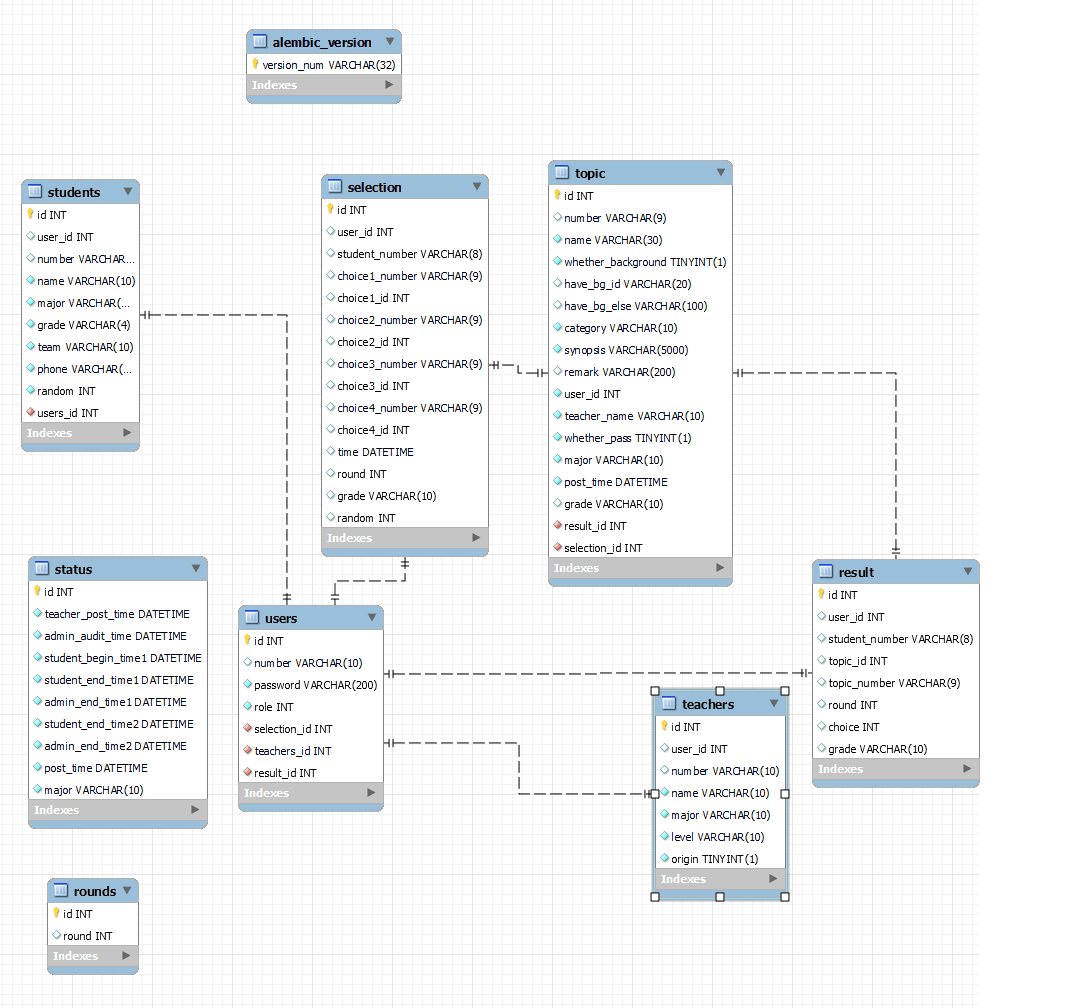
\includegraphics[width=0.7\textwidth]{关系模型.png}
    \caption{关系模型}
    \label{fig:ER}
\end{figure}

\clearpage

\subsection{数据库设计}



\begin{table}[ht]
    \centering
    \caption{users表}
    \begin{tabular}{|c|c|}
        \hline
        列名          & 备注     \\
        \hline
        id          & 自增主键id \\
        \hline
        number(int) & 用户id   \\
        \hline
        password    & 用户密码   \\
        \hline
        role(int)   & 用户权限   \\
        \hline
    \end{tabular}
    
    \label{tab:users}
\end{table}


\begin{table}[ht]
    \centering
    \caption{teachers表}
    \begin{tabular}{|c|c|}
        \hline
        列属性           & 备注               \\
        \hline
        id            & 自增主键id           \\
        \hline
        user\_id(int) & users外键id        \\
        \hline
        number(str)   & 教师工号             \\
        \hline
        name(str)     & 教师姓名             \\
        \hline
        major(str)    & 教师专业             \\
        \hline
        level(str)    & 教师职称             \\
        \hline
        origin(bool)  & 教师是否来自校外,默认false \\
        \hline
    \end{tabular}
    
    \label{tab:teachers}
\end{table}


\begin{table}[ht]
    \centering
    \caption{students表}
    \begin{tabular}{|c|c|}
        \hline
        列属性           & 备注        \\
        \hline
        id            & 自增主键id    \\
        \hline
        user\_id(int) & users外键id \\
        \hline
        number(str)   & 学生学号      \\
        \hline
        name(str)     & 学生姓名      \\
        \hline
        major(str)    & 学生专业      \\
        \hline
        grade(str)    & 年级        \\
        \hline
        team(str)     & 班级        \\
        \hline
        phone(str)    & 电话号码      \\
        \hline
        random(int)   & 随机数       \\
        \hline
    \end{tabular}
    
    \label{tab:students}
\end{table}

\clearpage

\begin{table}[ht]
    \centering
    \caption{status表(储存各种时间相关的数据)管理员设置}
    \begin{tabular}{|c|c|}
        \hline
        列属性                             & 备注                       \\
        \hline
        id                              & 自增主键id                   \\
        \hline
        teacher\_post\_time(datatime)   & 教师提交题目截止时间/管理员审核题目开始时间   \\
        \hline
        admin\_audit\_time(datatime)    & 管理员审核题目截止时间/学生浏览题目开始时间   \\
        \hline
        student\_begin\_time1(datatime) & 学生第一次选题开始时间/学生浏览题目结束时间   \\
        \hline
        student\_end\_time1(datatime)   & 学生第一次选题截止时间/管理员第一次匹配开始时间 \\
        \hline
        admin\_end\_time1(datatime)     & 管理员第一次匹配截止时间/学生第二次选题开始时间 \\
        \hline
        student\_end\_time2(datatime)   & 学生第二次选题截止时间/管理员第二次匹配开始时间 \\
        \hline
        admin\_end\_time2               & 管理员第二次匹配截止时间             \\
        \hline
        post\_time(datatime)            & 当前提交时间                   \\
        \hline
        major(str)                      & 设置适用的专业                  \\
        \hline
    \end{tabular}
    
    \label{tab:status}
\end{table}

\begin{table}[ht]
    \centering
    \caption{topic表}
    \begin{tabular}{|c|c|}
        \hline
        列属性                       & 备注                    \\
        \hline
        id                        & 自增主键id                \\
        \hline
        number                    & 课题编号                  \\
        \hline
        name(str)                 & 课题名称                  \\
        \hline
        whether\_background(bool) & 是否有项目背景,default=false \\
        \hline
        have\_bg\_id(str)         & 有背景的项目id              \\
        \hline
        have\_bg\_else(str)       & 有背景的项目补充              \\
        \hline
        category(str)             & 课题性质(类别)              \\
        \hline
        synopsis(str)             & 课题简介                  \\
        \hline
        remark(str)               & 备注                    \\
        \hline
        user\_id(int)             & 教师ID                  \\
        \hline
        teacher\_name(str)        & 指导教师名称                \\
        \hline
        whether\_pass(bool)       & 是否审核通过,default=false  \\
        \hline
        major(str)                & 课题适用专业                \\
        \hline
        topic\_time(datatime)     & 课题提交时间                \\
        \hline
    \end{tabular}
   
    \label{tab:topic}
\end{table}

\clearpage

\begin{table}[ht]
    \centering
    \caption{selection表}
    \begin{tabular}{|c|c|}
        \hline
        列属性                  & 备注       \\
        \hline
        id                   & 自增主键id   \\
        \hline
        user\_id(int)        & 学生ID     \\
        \hline
        student\_number(str) & 学生学号     \\
        \hline
        choice1\_number(str) & 第一志愿课题编号 \\
        \hline
        choice1\_id(int)     & 第一志愿id   \\
        \hline
        choice2\_number(str) & 第二志愿课题编号 \\
        \hline
        choice2\_id(int)     & 第二志愿id   \\
        \hline
        choice3\_number(str) & 第三志愿课题编号 \\
        \hline
        choice3\_id(int)     & 第三志愿id   \\
        \hline
        choice4\_number(str) & 第四志愿课题编号 \\
        \hline
        choice4\_id(int)     & 第四志愿id   \\
        \hline
        time(DateTime)       & 选题时间     \\
        \hline
        round(str)           & 第几轮选题    \\
        \hline
    \end{tabular}
    
    \label{tab:selection}
\end{table}

\begin{table}[ht]
    \centering
    \caption{result表}
    \begin{tabular}{|c|c|}
        \hline
        列属性                  & 备注     \\
        \hline
        id                   & 自增主键id \\
        \hline
        user\_id(int)        & 学生ID   \\
        \hline
        student\_number(str) & 学生学号   \\
        \hline
        topic\_id(int)       & 课题ID   \\
        \hline
        topic\_number(str)   & 课题编号   \\
        \hline
        round(str)           & 选中轮次   \\
        \hline
        choice(str)          & 选中志愿   \\
        \hline
    \end{tabular}
    
    \label{tab:result}
\end{table}

\clearpage